\documentclass[11pt]{scrartcl}
\usepackage[T1]{fontenc}
\usepackage[a4paper, left=3cm, right=2cm, top=2cm, bottom=2cm]{geometry}
\usepackage[activate]{pdfcprot}
\usepackage[ngerman]{babel}
\usepackage[parfill]{parskip}
\usepackage[utf8]{inputenc}
\usepackage{kurier}
\usepackage{amsmath}
\usepackage{amssymb}
\usepackage{xcolor}
\usepackage{epstopdf}
\usepackage{txfonts}
\usepackage{fancyhdr}
\usepackage{graphicx}
\usepackage{prettyref}
\usepackage{hyperref}
\usepackage{eurosym}
\usepackage{setspace}
\usepackage{units}
\usepackage{eso-pic,graphicx}
\usepackage{icomma}
\usepackage{pdfpages}

\definecolor{darkblue}{rgb}{0,0,.5}
\hypersetup{pdftex=true, colorlinks=true, breaklinks=false, linkcolor=black, menucolor=black, pagecolor=black, urlcolor=darkblue}



\setlength{\columnsep}{2cm}


\newcommand{\arcsinh}{\mathrm{arcsinh}}
\newcommand{\asinh}{\mathrm{arcsinh}}
\newcommand{\ergebnis}{\textcolor{red}{\mathrm{Ergebnis}}}
\newcommand{\fehlt}{\textcolor{red}{Hier fehlen noch Inhalte.}}
\newcommand{\betanotice}{\textcolor{red}{Diese Aufgaben sind noch nicht in der Übung kontrolliert worden. Es sind lediglich meine Überlegungen und Lösungsansätze zu den Aufgaben. Es können Fehler enthalten sein!!! Das Dokument wird fortwährend aktualisiert und erst wenn das \textcolor{black}{beta} aus dem Dateinamen verschwindet ist es endgültig.}}
\newcommand{\half}{\frac{1}{2}}
\renewcommand{\d}{\, \mathrm d}
\newcommand{\punkte}{\textcolor{white}{xxxxx}}
\newcommand{\p}{\, \partial}
\newcommand{\dd}[1]{\item[#1] \hfill \\}

\renewcommand{\familydefault}{\sfdefault}
\renewcommand\thesection{}
\renewcommand\thesubsection{}
\renewcommand\thesubsubsection{}


\newcommand{\themodul}{Halbleiter und Nanotechnologie}
\newcommand{\thetutor}{Prof. Förster}
\newcommand{\theuebung}{Übung 3}

\pagestyle{fancy}
\fancyhead[L]{\footnotesize{C. Hansen}}
\chead{\thepage}
\rhead{}
\lfoot{}
\cfoot{}
\rfoot{}

\title{\themodul{}, \theuebung{}, \thetutor}


\author{Christoph Hansen \\ {\small \href{mailto:chris@university-material.de}{chris@university-material.de}} }

\date{}


\begin{document}

\maketitle

Dieser Text ist unter dieser \href{http://creativecommons.org/licenses/by-nc-sa/4.0/}{Creative Commons} Lizenz veröffentlicht.

\textcolor{red}{Ich erhebe keinen Anspruch auf Vollständigkeit oder Richtigkeit. Falls ihr Fehler findet oder etwas fehlt, dann meldet euch bitte über den Emailkontakt.}

\tableofcontents


\newpage



\section{Aufgabe 1}

\subsection*{a)}

\begin{align*}
C' &= \frac{\epsilon_0 \epsilon_R}{w} \\
\Leftrightarrow w &= \frac{\epsilon_0 \epsilon_R}{C'} = \frac{12,9 \cdot 8,85 \cdot 10^{-12}}{10^{-3}} = \unit[114]{nm}
\end{align*}


\subsection*{b)}

\begin{align*}
w &= \sqrt{\frac{2 \epsilon_r \cdot \epsilon_0 \cdot \left( V_{bi} + V_R \right)}{e N_d}} \\
\Leftrightarrow V_{bi} + V_R &= \frac{w^2 e N_d}{2 \epsilon_r \epsilon_0} \\
\Leftrightarrow V_R &= -0,6 + \frac{w^2 e N_d}{2 \epsilon_r \epsilon_0} \\
&= -0,6 + \frac{\left( 114 \cdot 10^{-19} \right)^2 \cdot 1,6 \cdot 10^{-19} \cdot 10^{23}}{12,9 \cdot 8,85 \cdot 10^{-12}} = \unit[0,31]{V}
\end{align*}


\subsection*{c)}

Hier gilt $n = N_d$. Zur Anschaulichkeit ein Bild:

\begin{figure}[h]
	\centering
	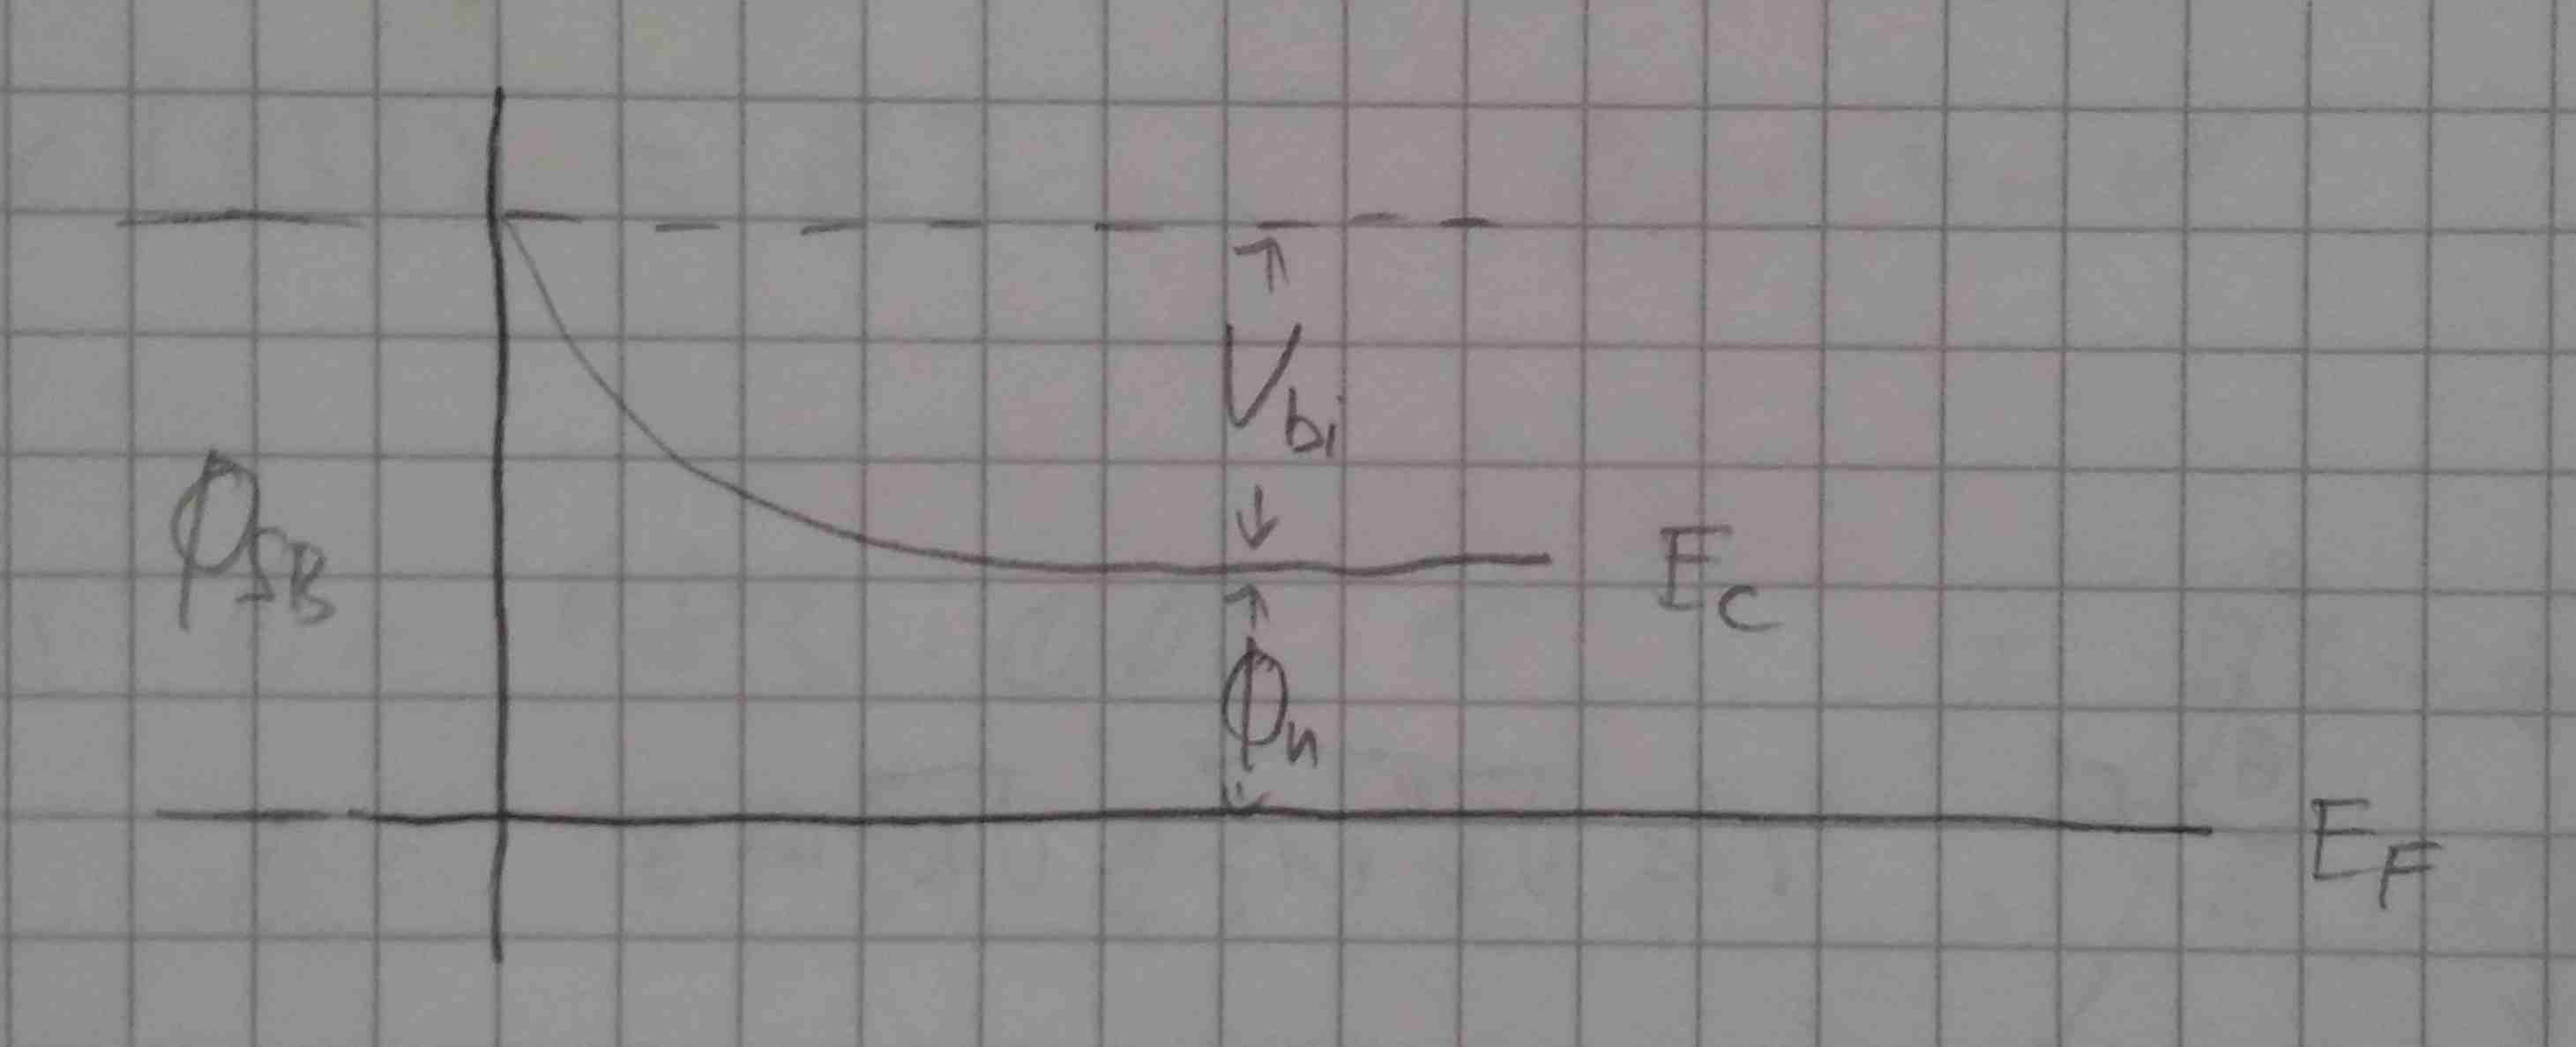
\includegraphics[scale=0.15]{A1_1.jpg}
\end{figure}


\begin{align*}
n &= N_c \cdot e^{- \frac{E_c - E_F}{kT}} \\
\Leftrightarrow \ln\left( \frac{n}{N_c} \right) &= - \frac{\phi_n e}{kT} \\
\Leftrightarrow \phi_n &= \frac{kT}{e} \cdot \ln \left( \frac{N_c}{n} \right) = \unit[38]{mV}
\intertext{Damit ist die Schottky Barriere:}
\phi_{SB} &= 0,038 + 0,6 = \unit[0,638]{mV}
\end{align*}



\section{Aufgabe 2}

\subsection*{a)}

\begin{align*}
j_s &= A^* T^2 \cdot e^{-e \cdot \frac{\phi_{SB} - \Delta \phi}{kT}}
\intertext{Wir vernachlässigen allerdings $\Delta \phi$, weil wir das E-Feld nicht kennen.}
&= 260 \cdot 300^2 \cdot e^{- \frac{0,72}{0,026}} = \unit[2,2 \cdot 10^{-5}]{A/cm^2}
\end{align*}

\subsection*{b)}

\begin{align*}
I_S &= j_s \cdot A = 2,2 \cdot 10^{-5} \cdot 10^{-6} = \unit[22 \cdot 10^{-12}]{A}
\end{align*}


\subsection*{c)}

Diese Teilaufgabe ist eigentlich falsch, da wie den Serienwiderstand nicht berücksichtigen!

\begin{align*}
I &= I_S \cdot \left( e^{\frac{U}{U_T}} - 1 \right) \\
\frac{U}{U_T} &= \ln \left( \frac{I}{I_s} + 1 \right) \\
\Leftrightarrow U &= U_T \cdot \ln \left( \frac{20 \cdot 10^{-3}}{22 \cdot 10^{-12}} + 1 \right) = \unit[0,52]{V}
\end{align*}

\newpage

\section{Aufgabe 3}

\subsection*{a)}

\begin{figure}[h]
	\centering
	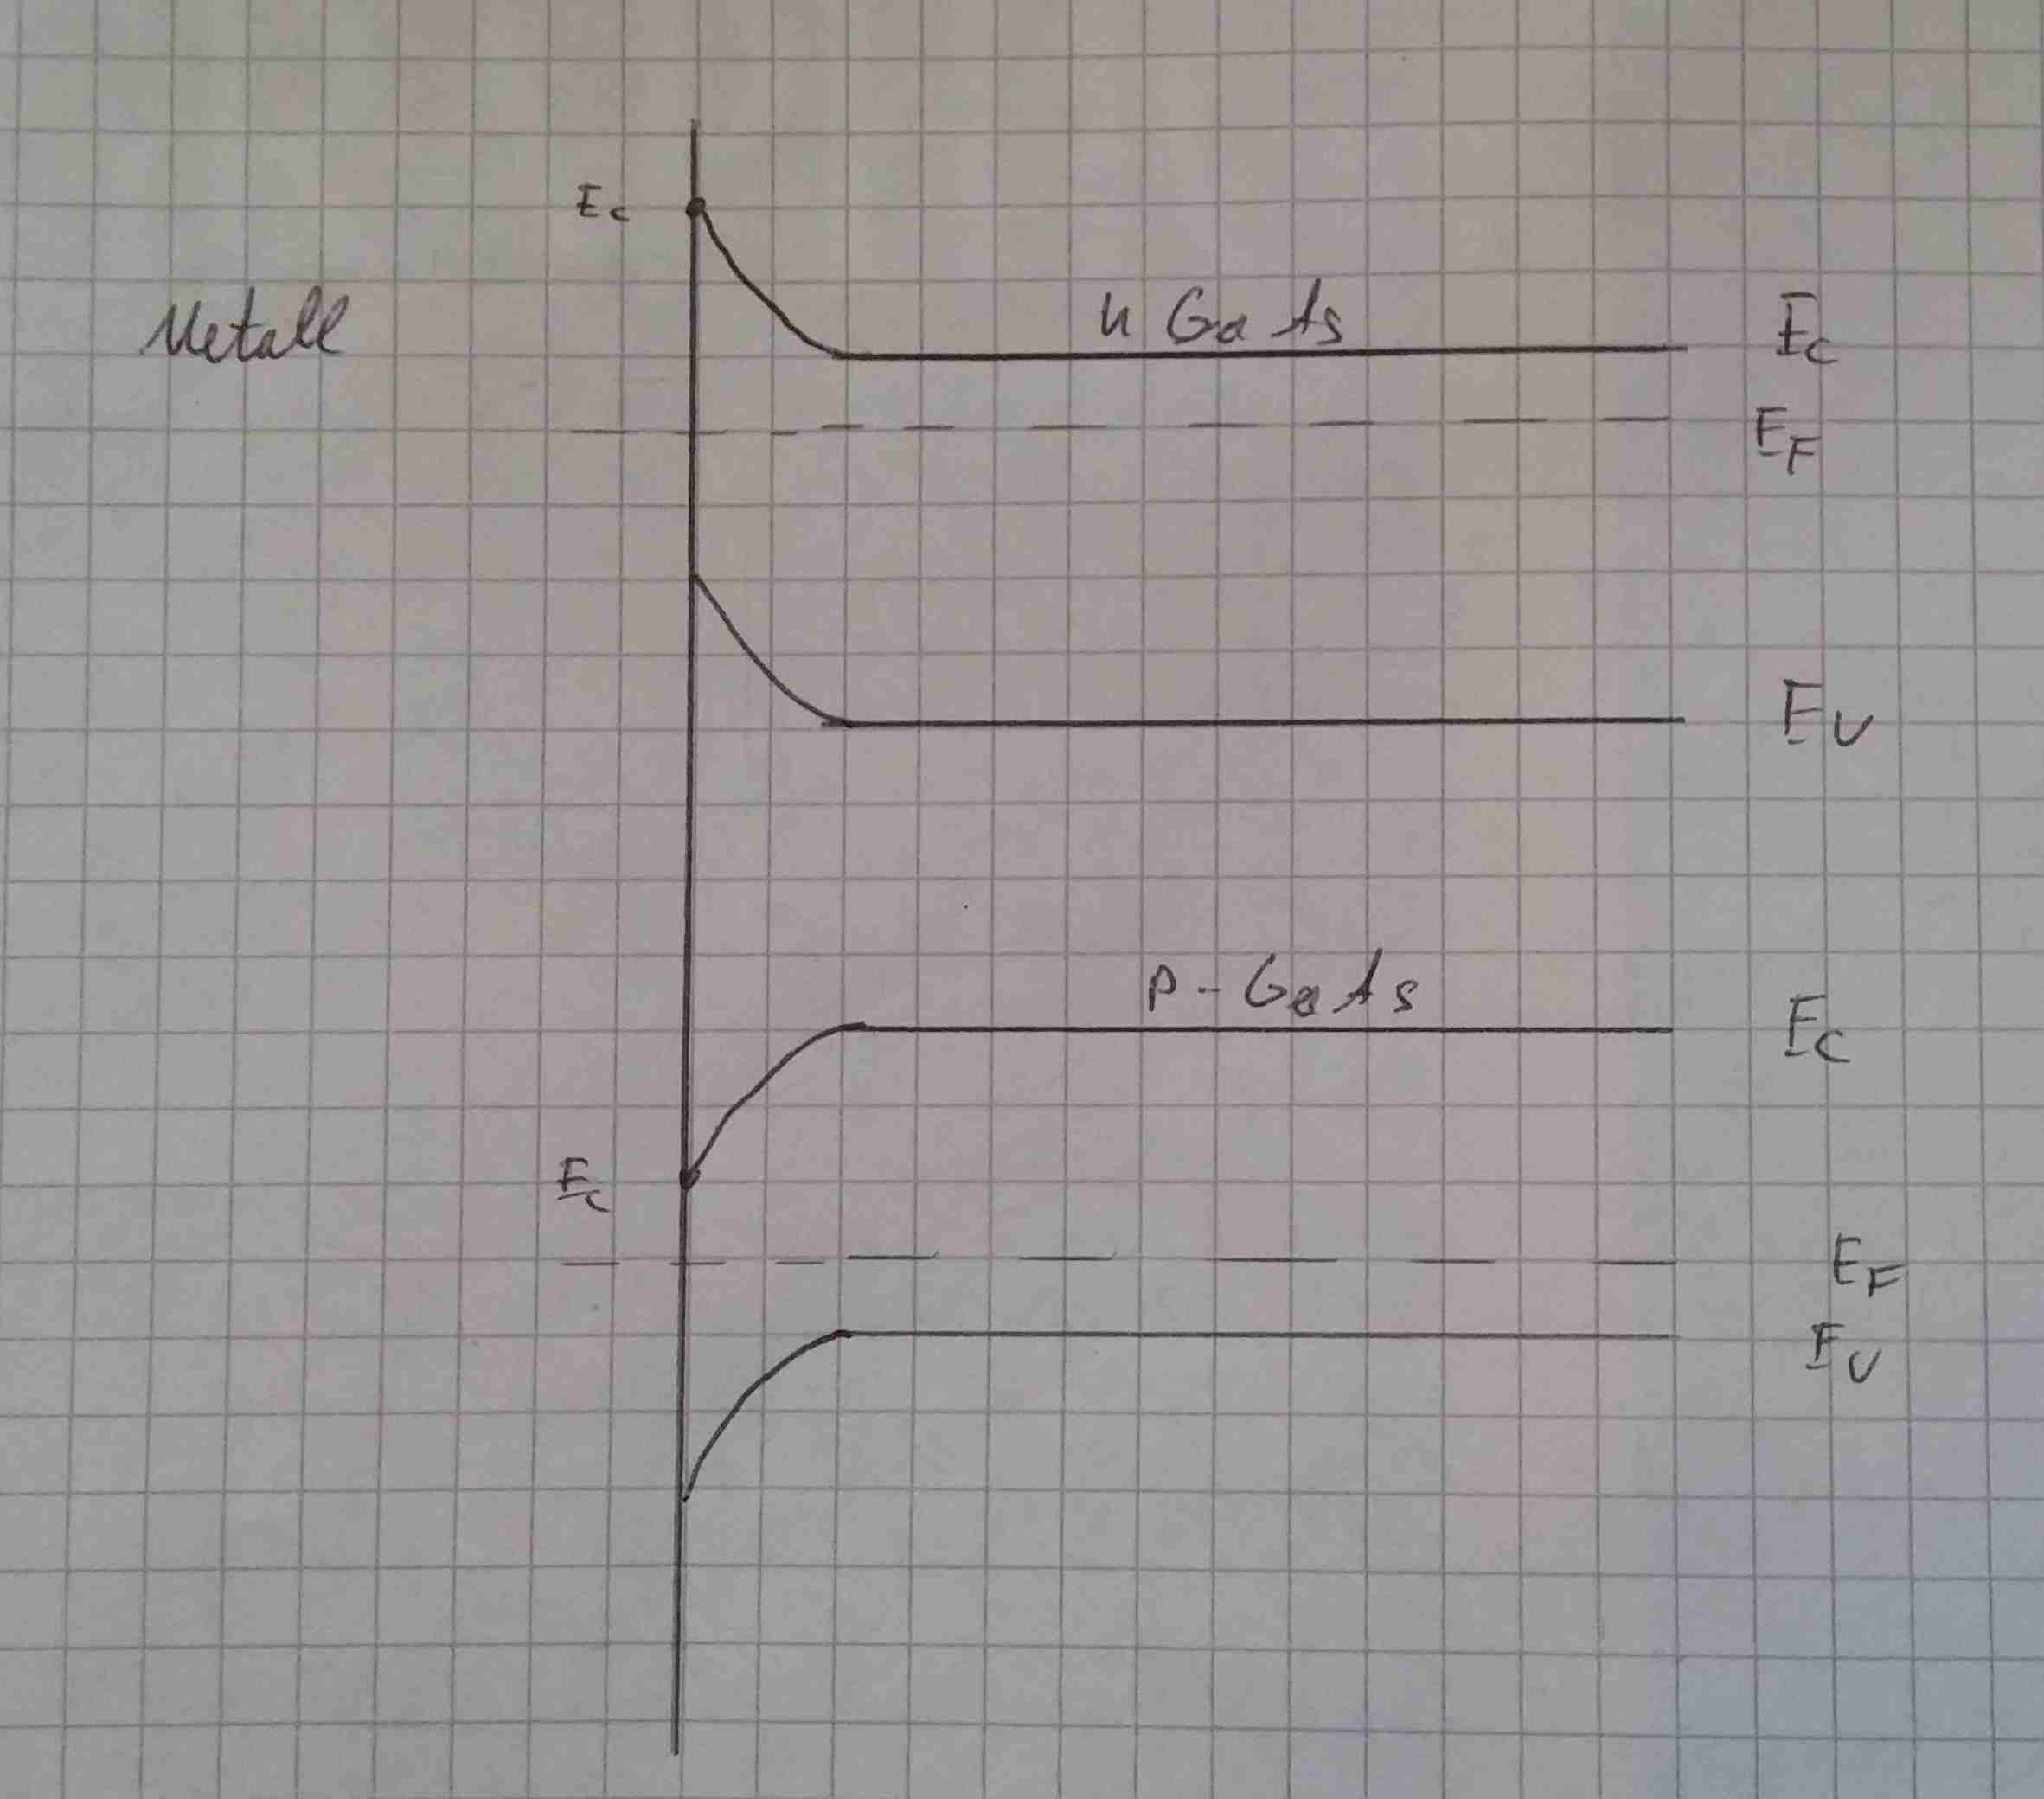
\includegraphics[scale=0.15]{A3_1.jpg}
\end{figure}

\newpage

\subsection*{b)}


\begin{figure}[h]
	\centering
	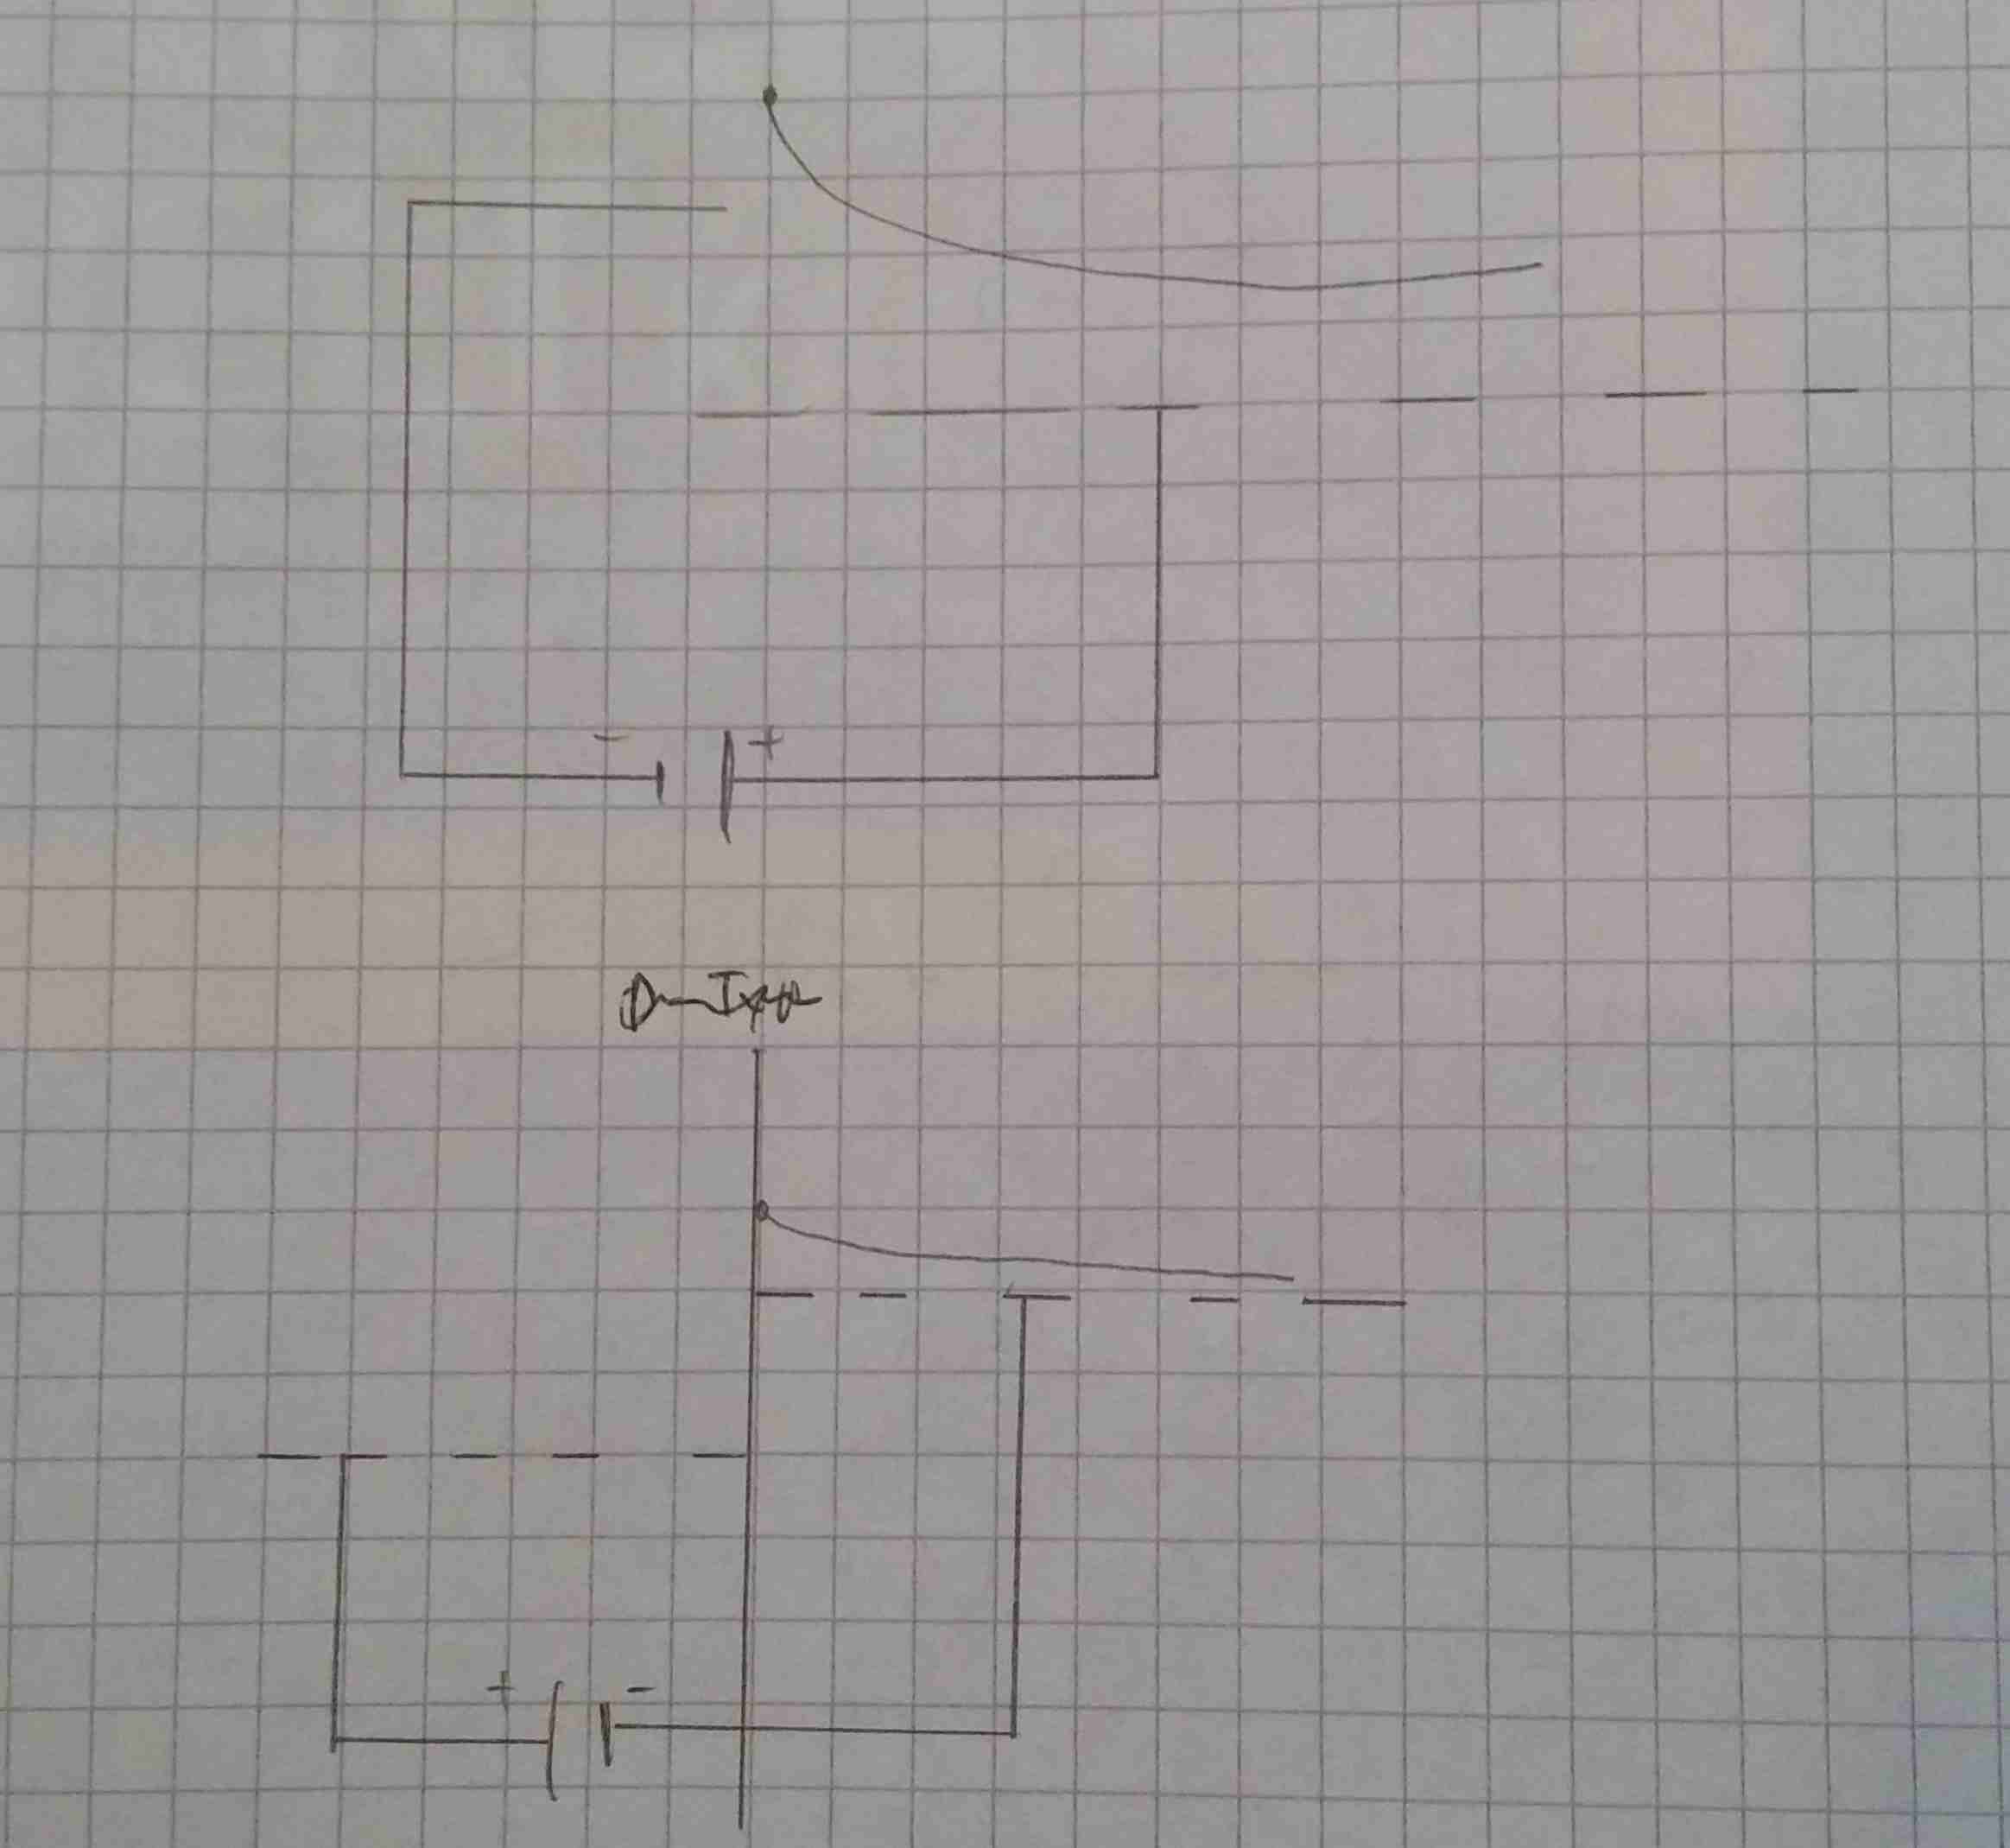
\includegraphics[scale=0.13]{A3_2.jpg}
	\caption{n-Typ}
\end{figure}


\begin{figure}[h]
	\centering
	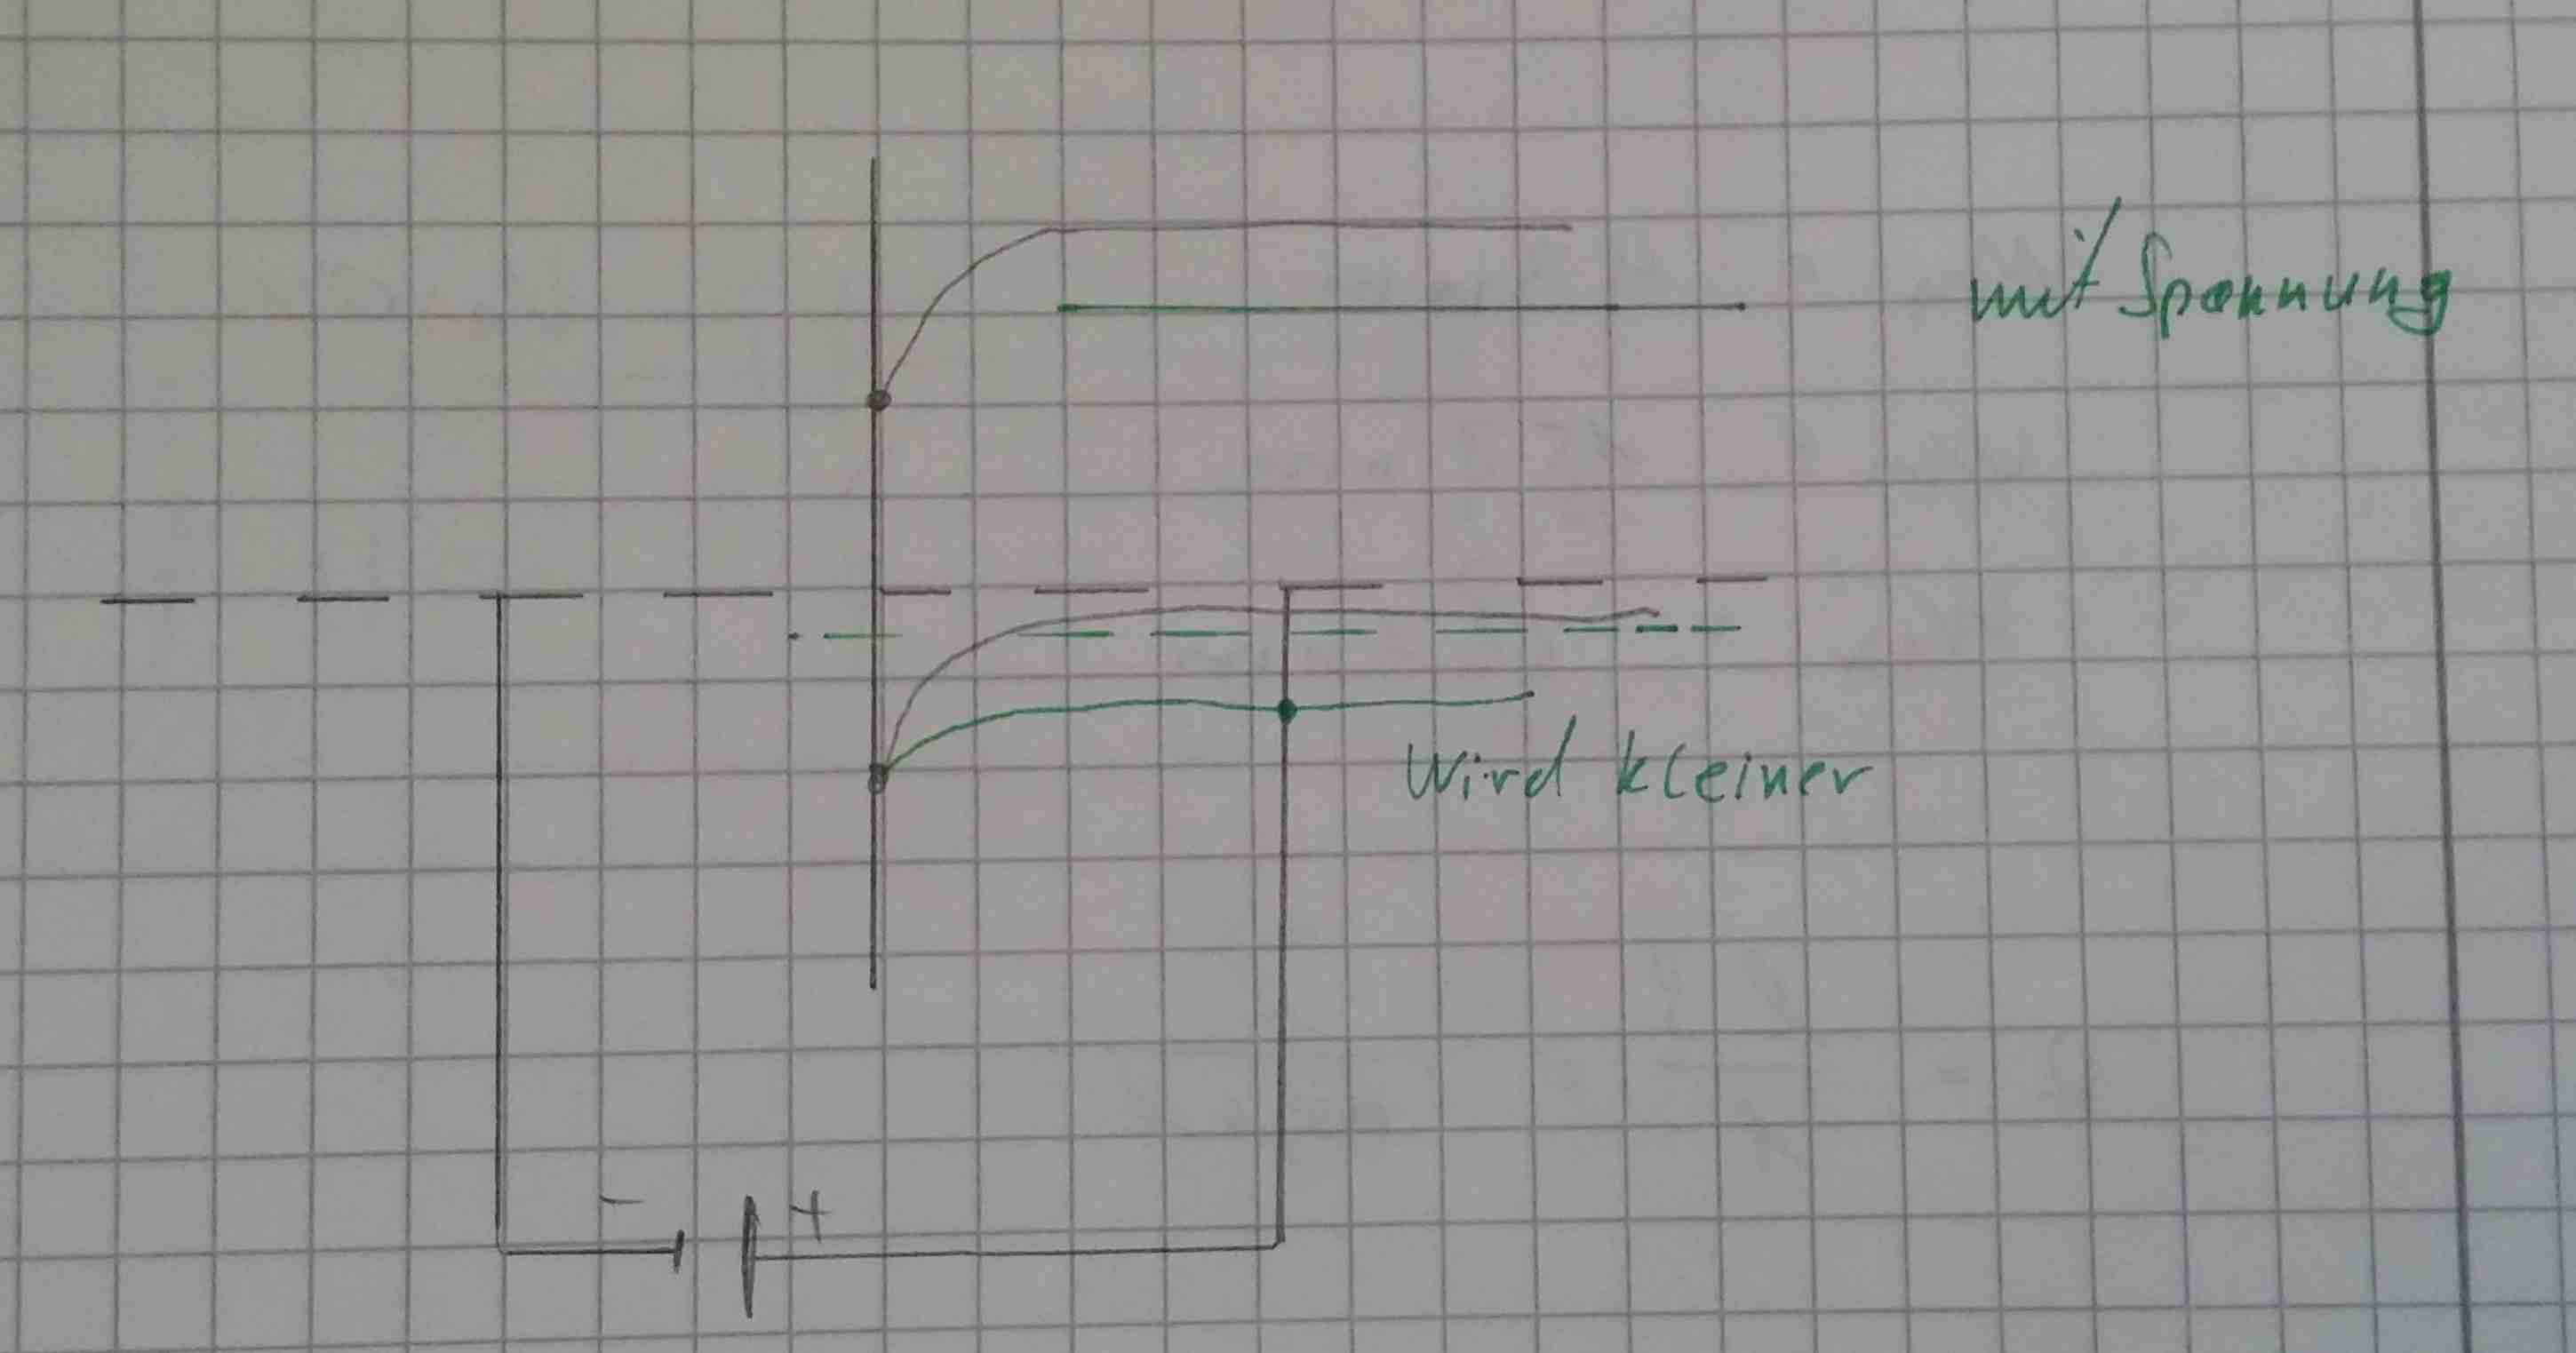
\includegraphics[scale=0.13]{A3_3.jpg}
	\caption{p-Typ}
\end{figure}

\newpage

\subsection*{c)}

Wir rechnen anders als in der Aufgabenstellung mit $V_{bi} = \unit[0,6]{V}$

\begin{figure}[h]
	\centering
	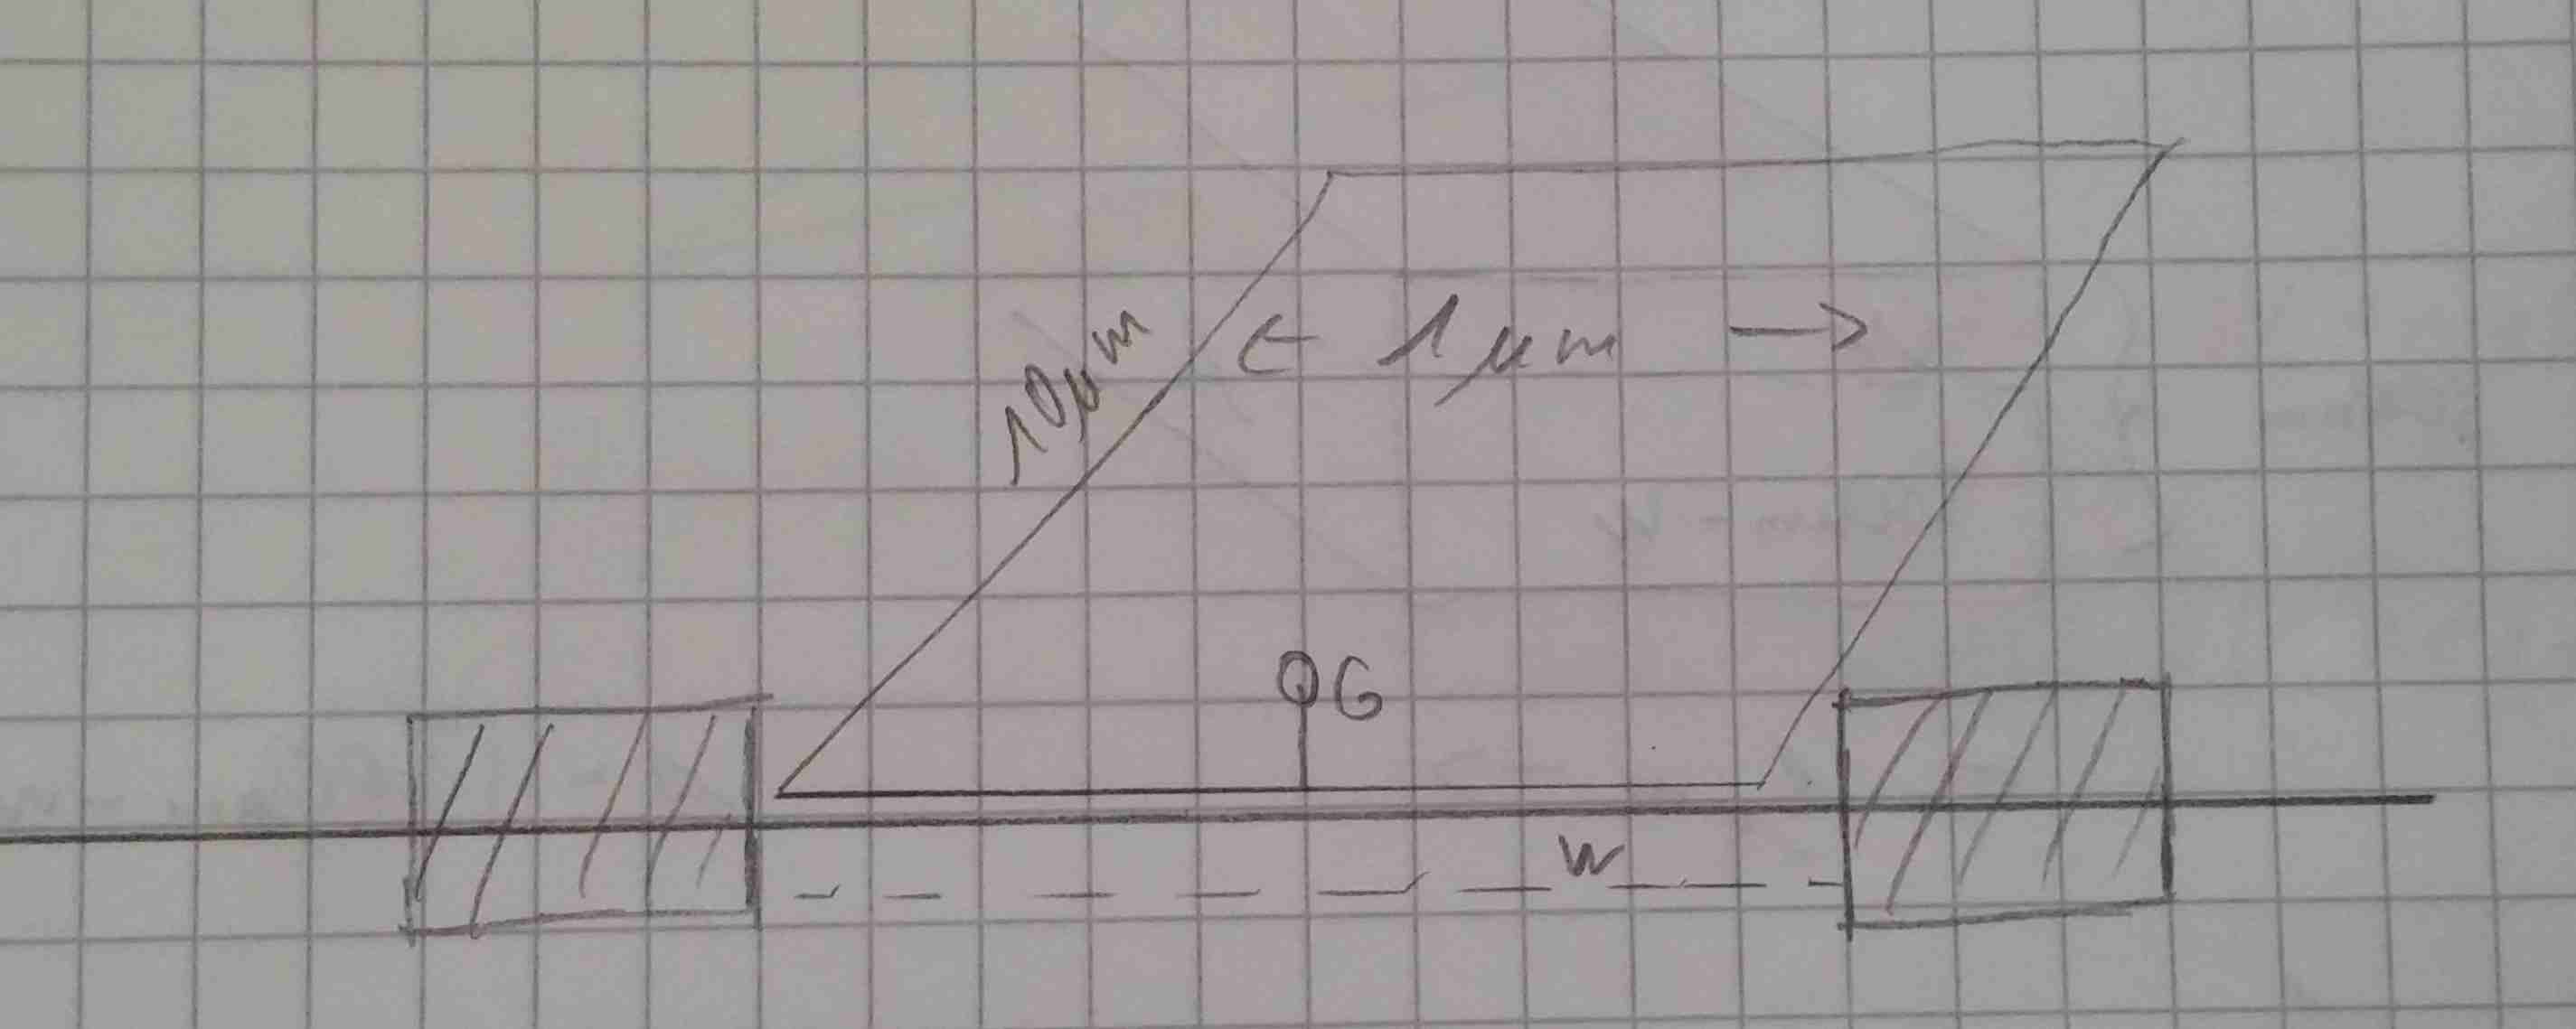
\includegraphics[scale=0.13]{A3_4.jpg}
\end{figure}


\subsubsection{c1)}


\begin{align*}
w &= \sqrt{\frac{2 \epsilon_r \cdot \epsilon_0 \cdot \left( V_{bi} + V_R \right)}{e N_d}} = \sqrt{\frac{2 \cdot 8,85 \cdot 10^{-12} \cdot 12,9 \cdot 0,6}{1,6 \cdot 10^{-19} \cdot 10^{23}}} = \unit[93]{nm}
\end{align*}


\subsubsection{c2)}

\begin{align*}
w &= \sqrt{\frac{2 \epsilon_r \cdot \epsilon_0 \cdot \left( V_{bi} + V_R \right)}{e N_d}} \\
\Leftrightarrow V_R &= \frac{\left( 300 \cdot 10^{-9} \right)^2 \cdot 1,6 \cdot 10^{-19} \cdot 10^{23}}{2 \cdot 12,9 \cdot 8,85 \cdot 10^{-12}} = \unit[5,7]{V}
\end{align*}

\subsection*{d)}

Wir berechnen die Dicken für die einzelnen Reversespannungen:

\begin{align*}
w(0) &= \unit[93]{nm} \\
w(1) &= \unit[152]{nm} \\
w(3) &= \unit[227]{nm} 
\intertext{Den Widerstand bestimmen wir dann so:}
R &= \frac{l \rho}{A} = \frac{l}{ne \mu A}
\end{align*}

\newpage

Anschaulich sieht das ungefähr so aus:

\begin{figure}[h]
	\centering
	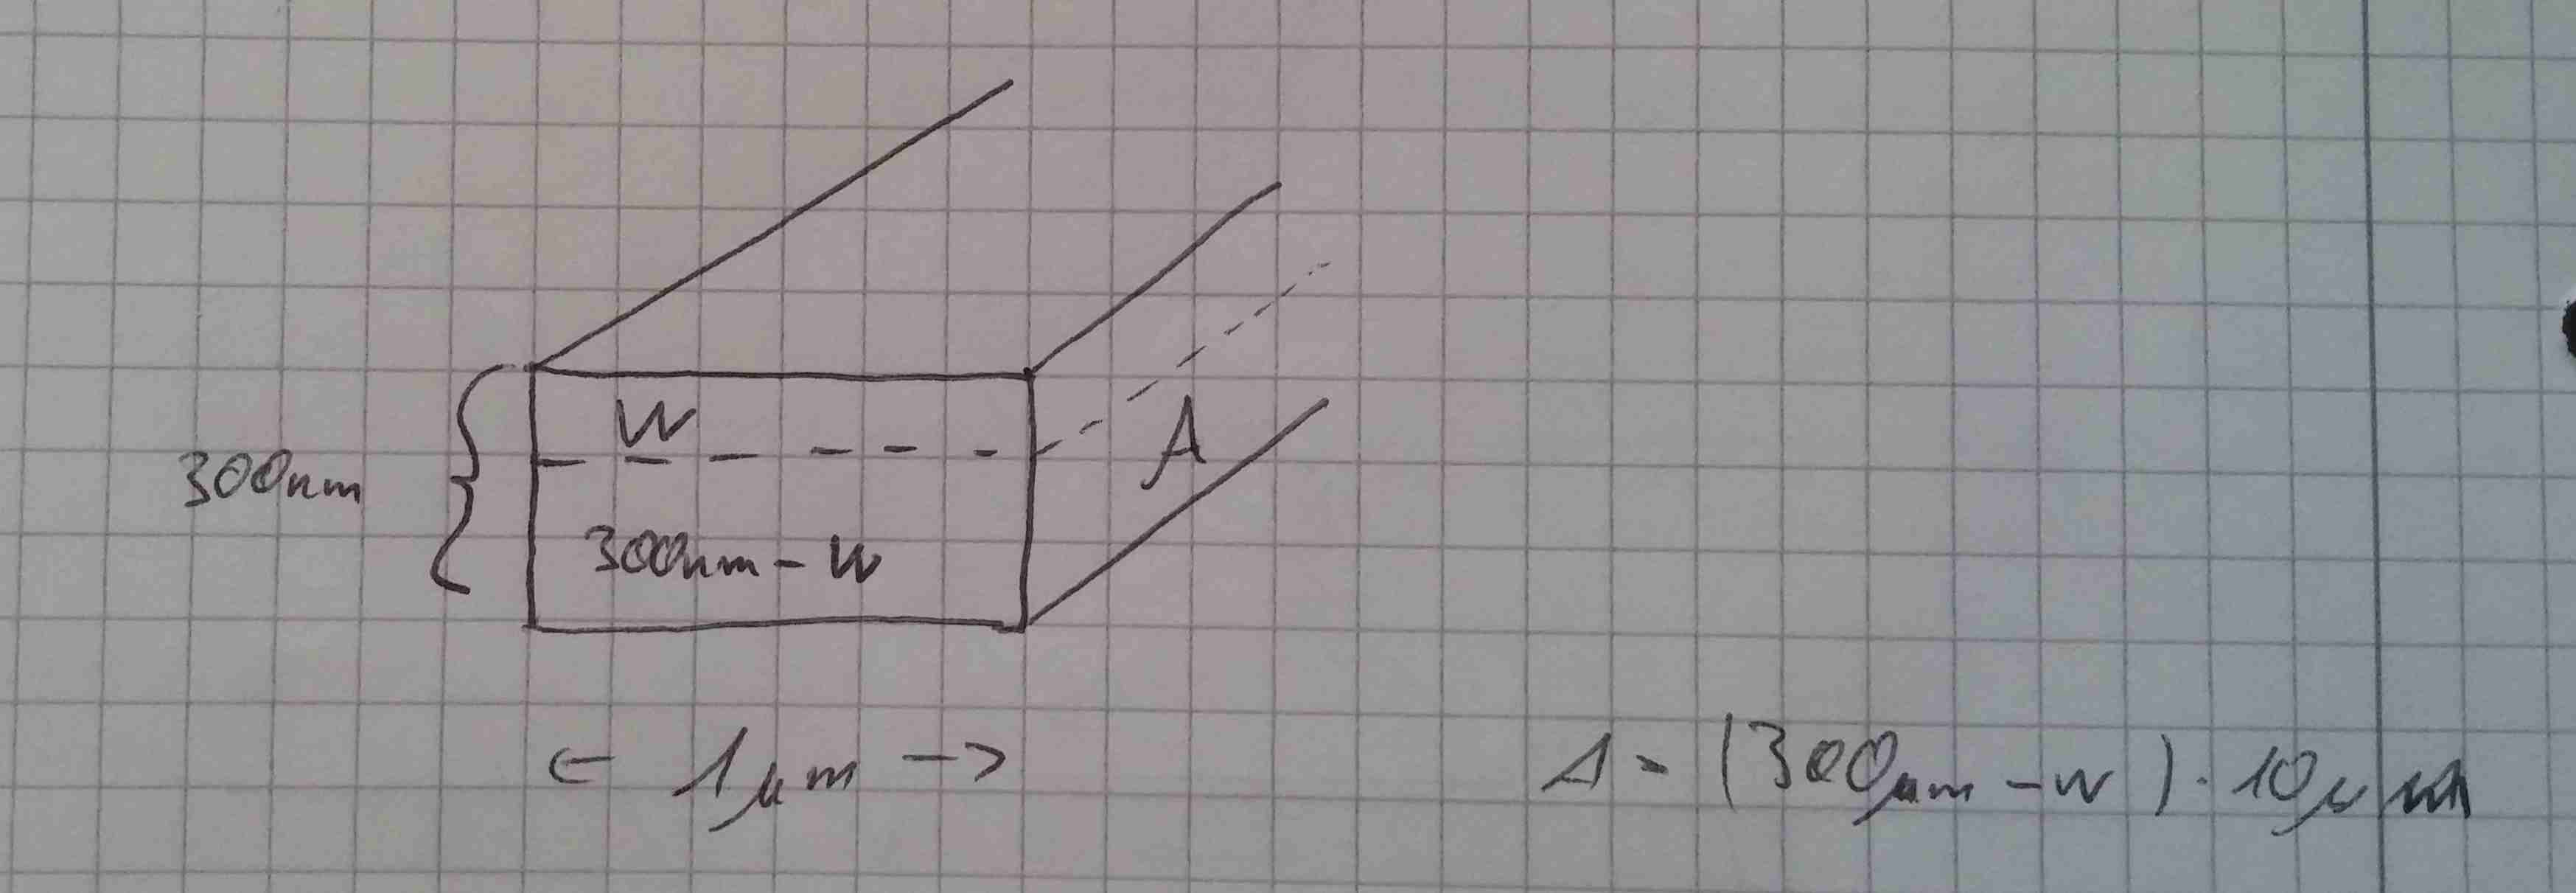
\includegraphics[scale=0.1]{A3_5.jpg}
\end{figure}

Die Widerstände ergeben sich dann zu:

\begin{align*}
R(0) &= \frac{10^{-6}}{10^{23} \cdot 1,6 \cdot 10^{-19} \cdot 0,2 \cdot \left( 300 - 93 \right) \cdot 10^{-9} \cdot 10^{-5}} = \unit[151]{\Omega} \\
R(1) &= \frac{10^{-6}}{10^{23} \cdot 1,6 \cdot 10^{-19} \cdot 0,2 \cdot \left( 300 - 152 \right) \cdot 10^{-9} \cdot 10^{-5}} = \unit[211]{\Omega} \\
R(3) &= \frac{10^{-6}}{10^{23} \cdot 1,6 \cdot 10^{-19} \cdot 0,2 \cdot \left( 300 - 227 \right) \cdot 10^{-9} \cdot 10^{-5}} = \unit[428]{\Omega} 
\intertext{Die Leitwerte sind dann:}
G(0) &= \unit[6,6 \cdot 10^{-3}]{1/\Omega} \\
G(1) &= \unit[4,74 \cdot 10^{-3}]{1/\Omega}\\
G(3) &= \unit[2,33 \cdot 10^{-3}]{1/\Omega}
\end{align*}

\newpage


\section{Aufgabe 4}

\subsection*{a)}

\begin{figure}[h]
	\centering
	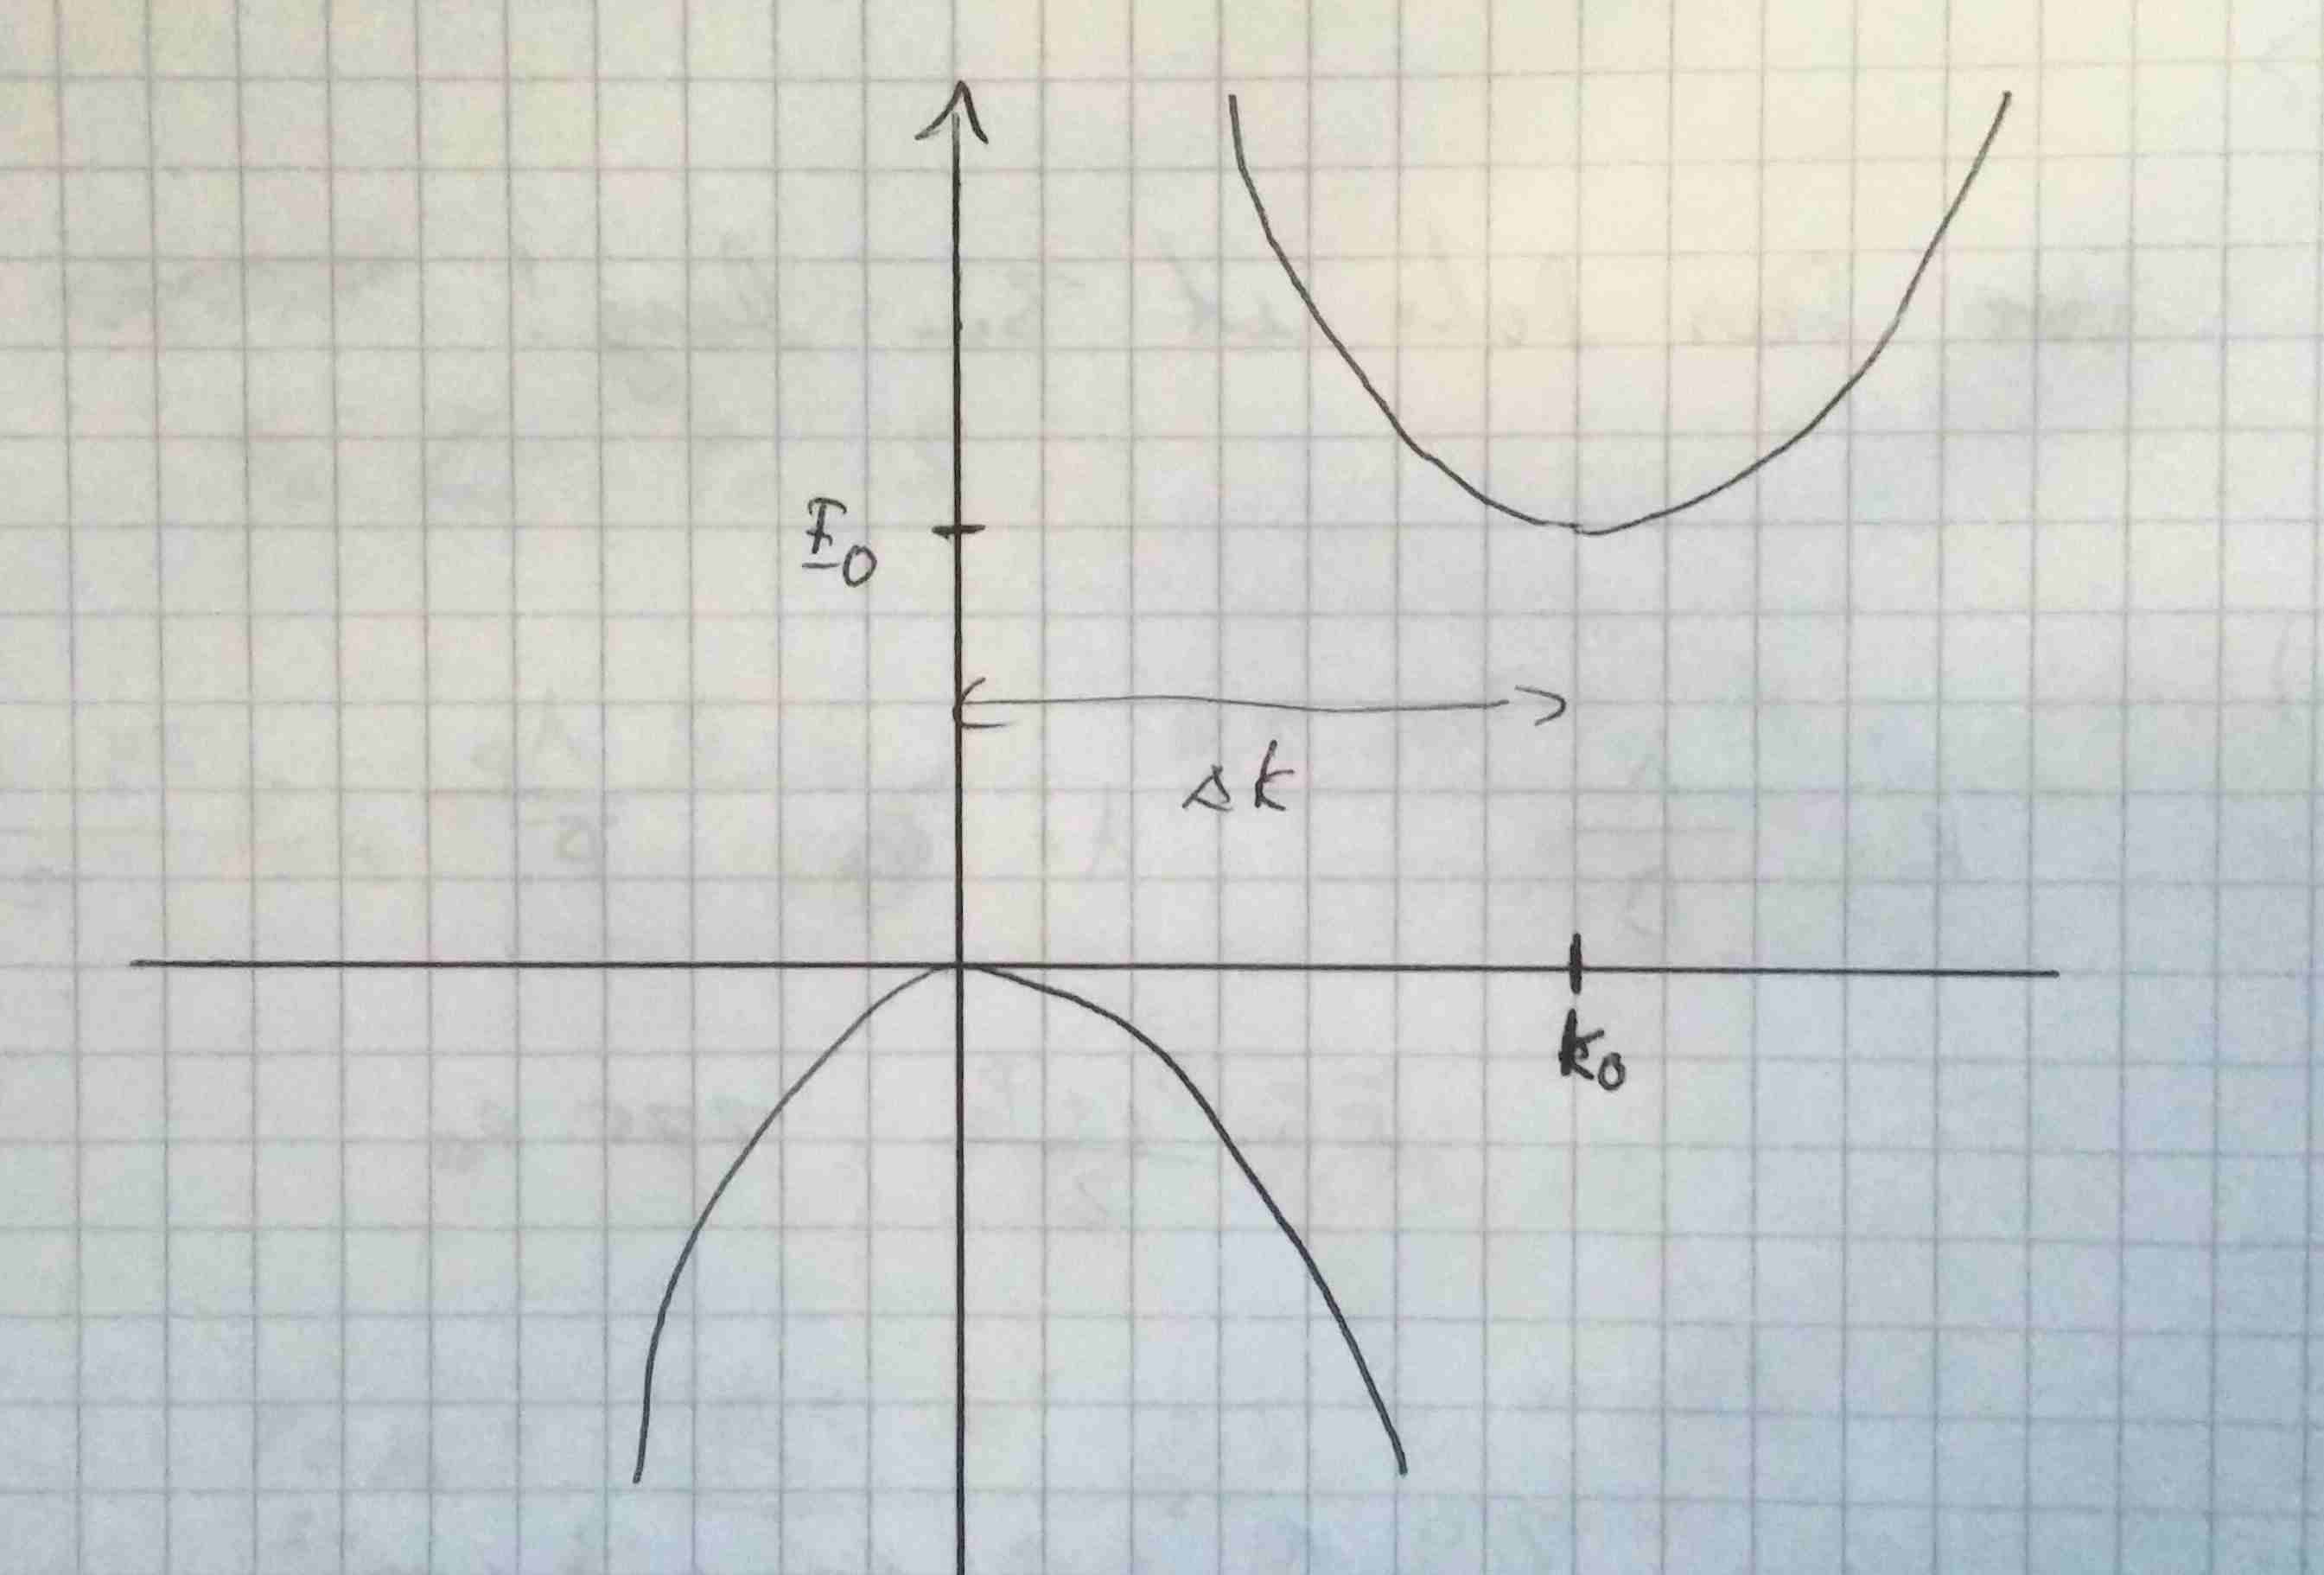
\includegraphics[scale=0.16]{A4_1.jpg}
\end{figure}


\subsection*{b)}

Die Raumladungszone wird nach rechts größer.


\subsection*{c)}

\begin{figure}[h]
	\centering
	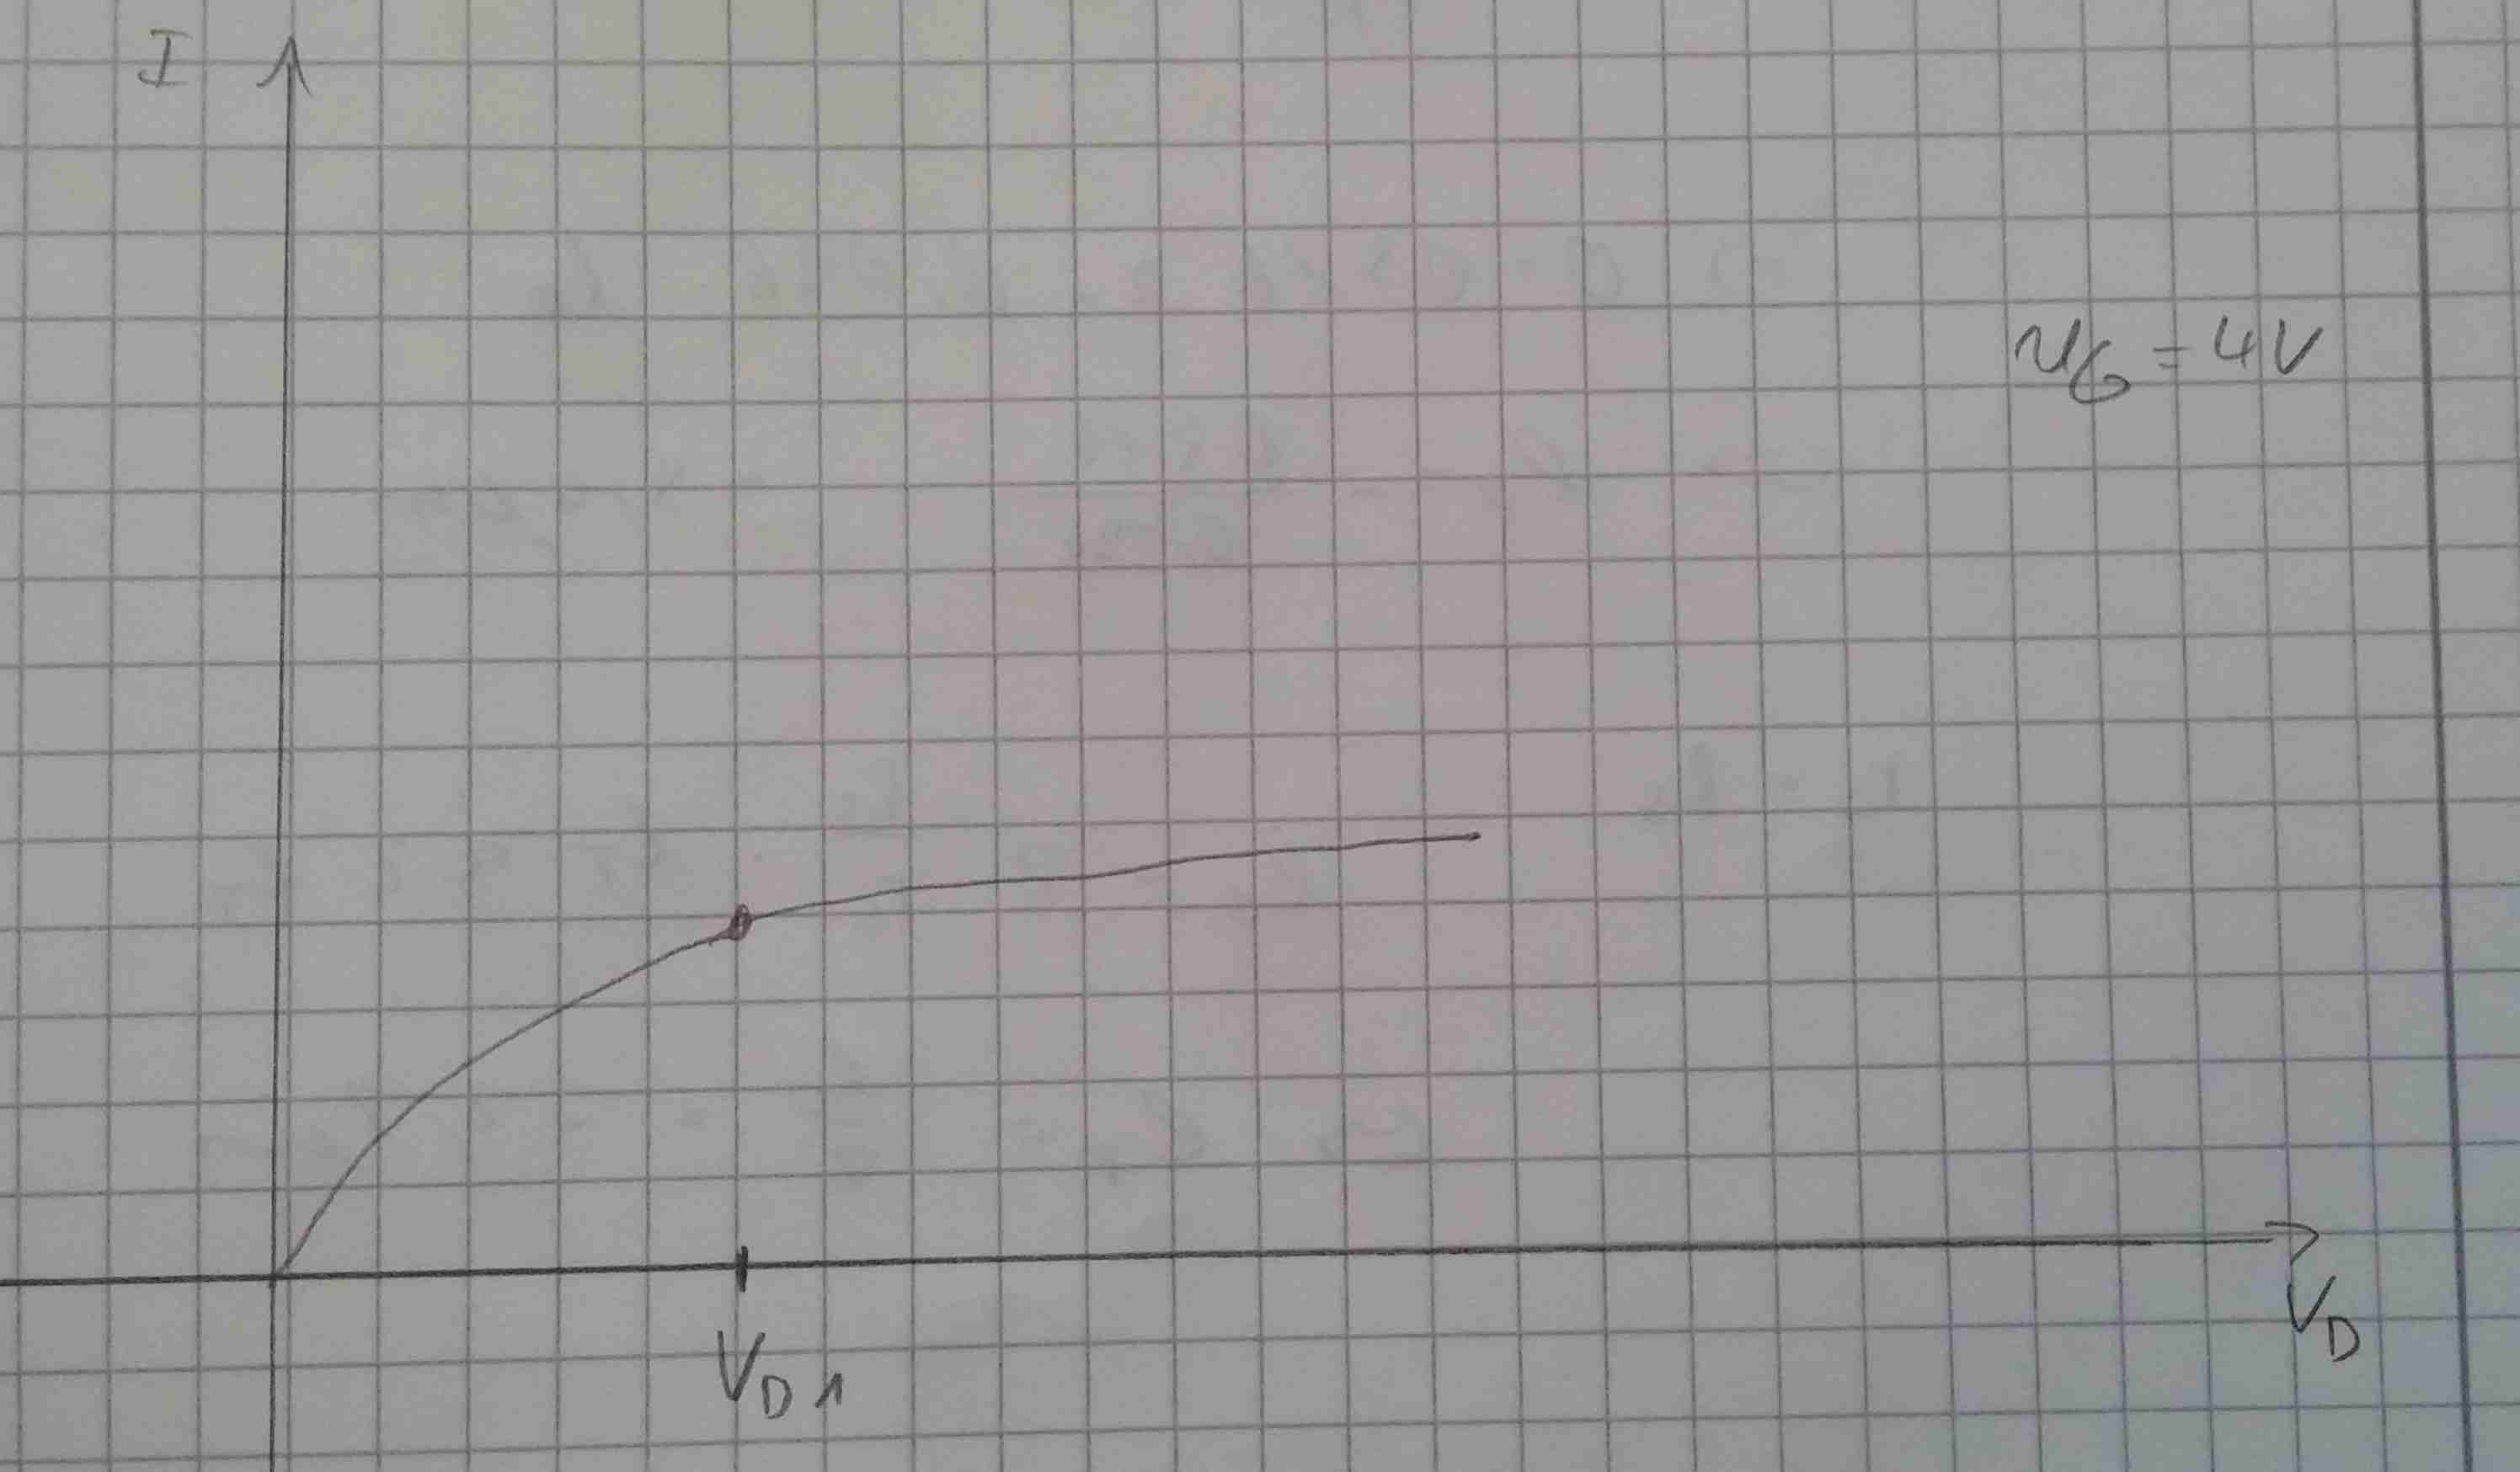
\includegraphics[scale=0.12]{A4_2.jpg}
\end{figure}



\section{Aufgabe 5}

\subsection*{a)}

\begin{figure}[h]
	\centering
	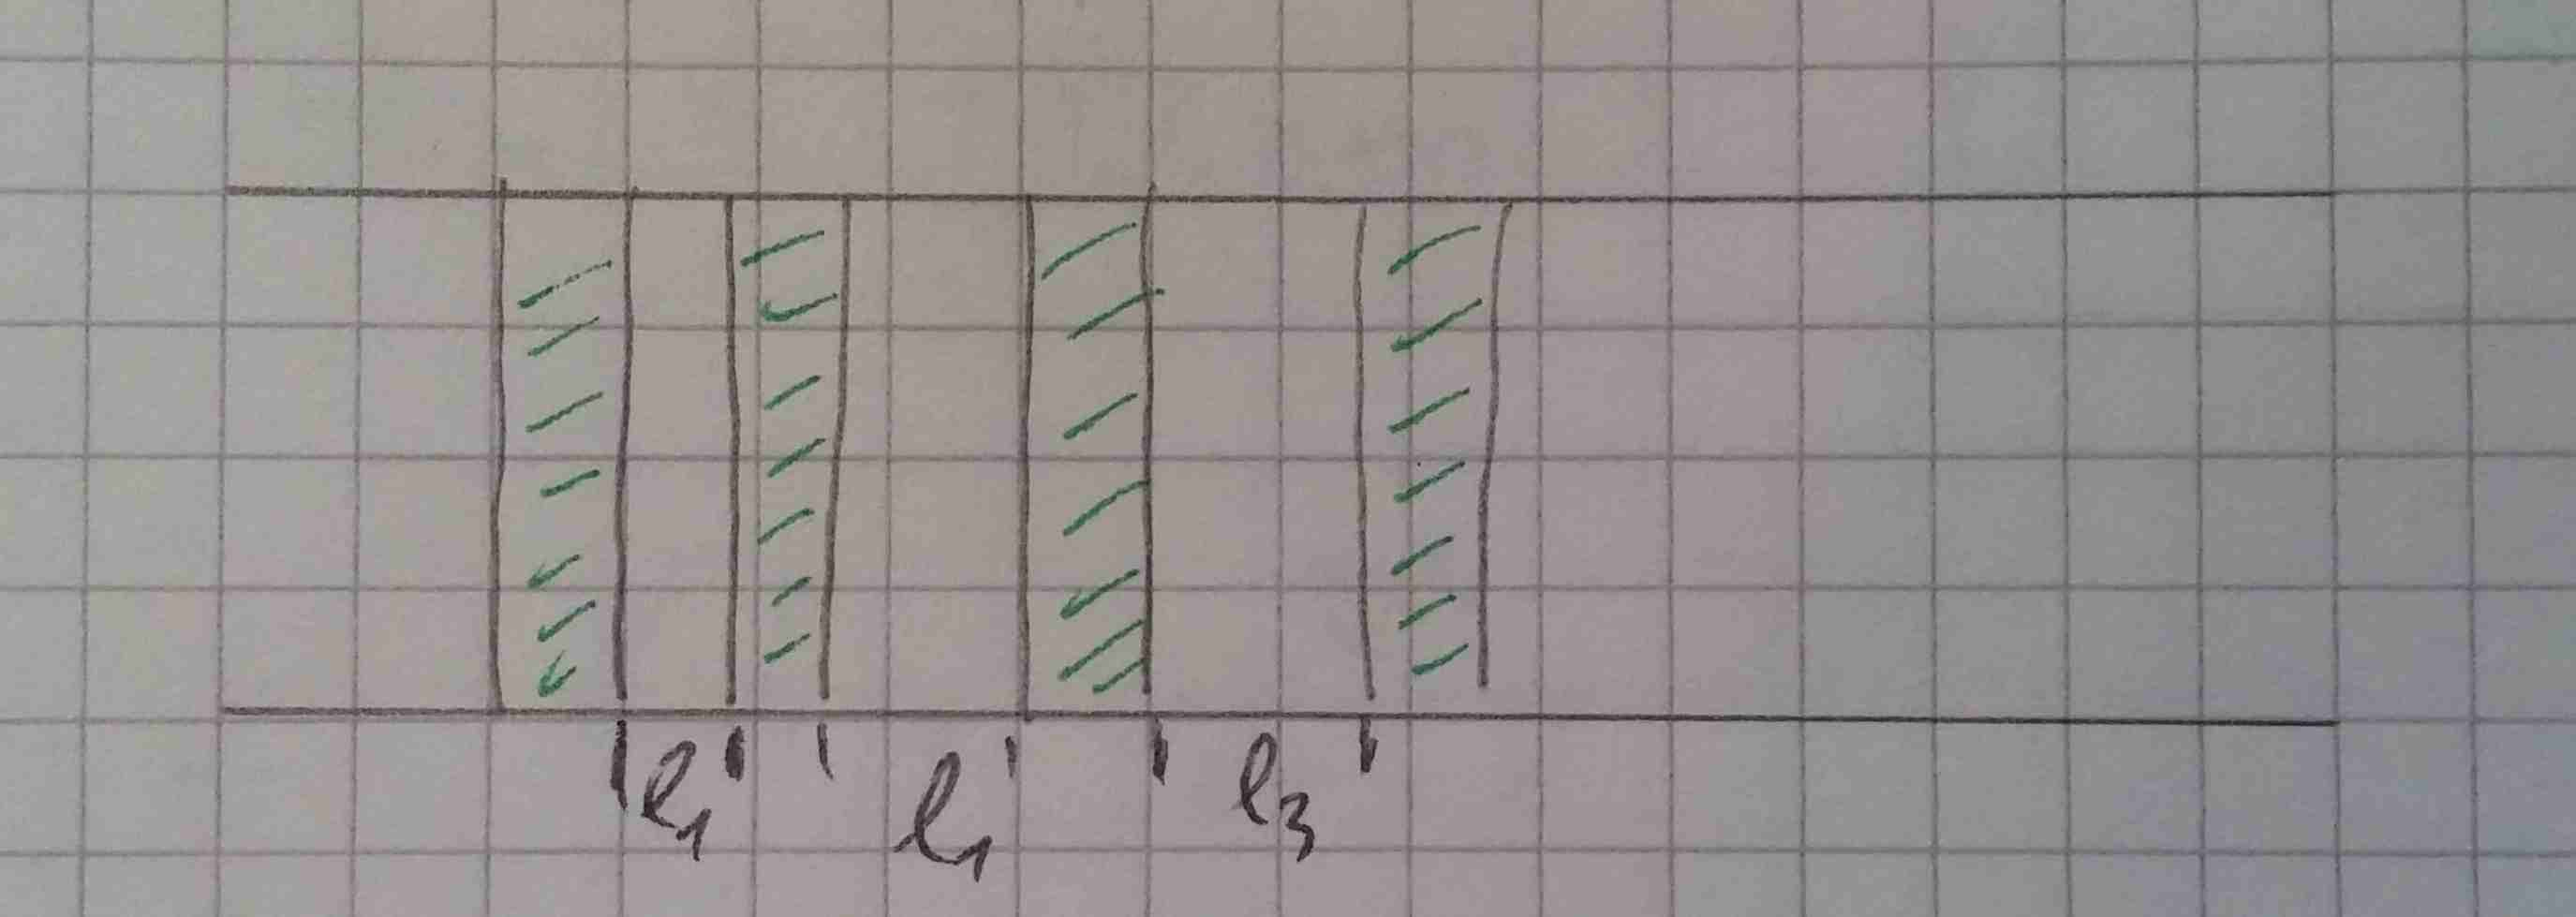
\includegraphics[scale=0.1]{A5_1.jpg}
\end{figure}

Es gilt das $2 R_C$, wenn $l_i = 0$

\begin{align*}
2 R_C &= 0,516 \\
\Leftrightarrow R_C &= \unit[0,258]{\Omega}
\end{align*}


\subsection*{b)}

Wir müssen zunächst $l_0$ bestimmen, dasmit wir dann $l_T$ berechnen können. $l_0$ ist der Schnittpunkt bei $R = 0$:

\begin{align*}
0 &= 0,516 + 0,096 \cdot l_0 \\
\Leftrightarrow l_0 &= - \frac{0,516}{0,096} = \unit[- 5,4]{\mu m}
\intertext{Wir setzen $r_s = R_s$ vorraus:}
l_0 &= 2 \cdot \frac{R_s}{r_s} \cdot l_T \approx 2 \cdot l_T \\
\Leftrightarrow l_T &= \frac{l_0}{2} = \unit[-2,7]{\mu m}
\intertext{Nun bestimmen wir noch die effektice Kontaktfläche:}
A_{eff} &= 10 \cdot 10^{-6} \cdot l_T = 10 \cdot 10^{-6} \cdot 2,7 \cdot 10^{-6} = \unit[27 \cdot 10^{-12}]{m^2}
\end{align*}


\subsection*{d)}

\begin{align*}
\rho_i &= R_c \cdot A = 0,258 \cdot 27 \cdot 10^{-12} = \unit[6,69 \cdot 10^{-12}]{\Omega \ m^2}
\end{align*}


\subsection*{e)}

\begin{align*}
R &= \frac{\rho \cdot e}{A} = \frac{6,69 \cdot 10^{-12}}{4 \cdot 0,5 \cdot 10^{-12}} = \unit[3,5]{\Omega}
\end{align*}





























\end{document}